\documentclass[addpoints]{exam}
\usepackage[utf8]{inputenc}
\usepackage[spanish]{babel}
\usepackage[T1]{fontenc}
\usepackage{charter}
\usepackage{amsmath}
\usepackage{amsfonts}
\usepackage{amssymb}
\usepackage{graphicx}
\usepackage{tikz}
\usepackage[outline]{contour} % glow around text
\usetikzlibrary{babel,calc,patterns,decorations.pathmorphing,decorations.markings,arrows.meta,shapes.geometric}
\usetikzlibrary{calc}
\tikzset{>=latex}
\contourlength{1.1pt}
\usepackage{tikz-3dplot}
\usepackage{multicol}
\usepackage{exam-randomizechoices}
\usepackage[left=1cm,right=1cm,top=2cm,bottom=2cm]{geometry}
\usepackage[font=small,labelfont={small,bf},margin=0.5cm,justification=justified]{caption}
\usepackage[font=small,labelfont={small,bf}]{subcaption}
\usepackage[italic,defaultmathsizes]{mathastext}
\usepackage{hyperref}
\usepackage{calculator}
\usepackage[breakable]{tcolorbox}
\usepackage{multirow}
\usepackage{tabularx}
\usepackage{cancel}
\usepackage{tipa}
\usepackage{enumerate}

%\pointpoints{punto}{puntos}
%\bonuspointpoints{punto extra}{puntos extra}

\renewcommand{\solutiontitle}{\textbf{Solución: }}
\renewcommand{\thequestion}{\bfseries\arabic{question}}

\newcommand{\sgn}{\mathop{\mathrm{sgn}}}
\newcommand{\diff}[0]{\mathrm{d}}
\newcommand{\fdiff}[2]{\frac{\mathrm{d} #1}{\mathrm{d} #2}}
\newcommand{\pdiff}[2]{\frac{\partial #1}{\partial #2}}
\newcommand{\fddiff}[2]{\frac{\mathrm{d^2} #1}{\mathrm{d} #2^2}}
\newcommand{\pddiff}[2]{\frac{\partial^2 #1}{\partial {#2}^2}}
\newcommand{\grado}[0]{^{\circ}}
\newcommand{\angulo}[3]{#1\grado \, #2' \, #3''}
\newcommand{\chel}[4]{^{#1}_{#2}\mbox{#3}^{#4}}
\newcommand{\valmed}[1]{\left\langle #1 \right\rangle}
\newcommand{\E}[1]{\times 10^{#1}}
\newcommand{\ver}[1]{\hat{\vec{#1}}}
\newcommand{\vecg}[1]{\boldsymbol{#1}}
\newcommand{\iu}{\mathrm{i}}
\newcommand{\norm}[1]{\left\vert\left\vert #1 \right\vert\right\vert}
\newcommand{\abs}[1]{\left\vert #1 \right\vert}
\newcommand{\tens}[1]{\mathbb{#1}}
\newcommand{\rr}{\mathbb{R}}
\newcommand{\un}[1]{\text{#1}}
\newcommand{\logoUNAHUR}{
\includegraphics[scale=0.35]{/home/shluna/UNAHUR/IAM/Apuntes/logo_unahur.png}}
\renewcommand{\arraystretch}{1.5}
\newcommand{\rta}{\textbf{Respuesta: }}
\newcommand{\rtas}{\textbf{Respuestas: }}
\newcommand{\ang}{110}
\newcommand{\angu}{-30}
\newcommand{\rad}{4}
\newcommand{\mg}{1}
\newcommand{\muc}{0.5}
\newcommand{\arc}[1]{{%
  \setbox9=\hbox{#1}%
  \ooalign{\resizebox{\wd9}{\height}{\texttoptiebar{\phantom{A}}}\cr#1}}}

  \colorlet{mydarkblue}{blue!40!black}
  \colorlet{myblue}{blue!30}
  \colorlet{myred}{red!65!black}
  \colorlet{vcol}{green!45!black}
  \colorlet{watercol}{blue!80!cyan!10!white}
  \colorlet{darkwatercol}{blue!80!cyan!80!black!30!white}
  \tikzstyle{water}=[draw=mydarkblue,top color=watercol!90,bottom color=watercol!90!black,middle color=watercol!50,shading angle=0]
  \tikzstyle{horizontal water}=[water,
    top color=watercol!90!black!90,bottom color=watercol!90!black!90,middle color=watercol!80,shading angle=0]
  \tikzstyle{dark water}=[draw=blue!20!black,top color=darkwatercol,bottom color=darkwatercol!80!black,middle color=darkwatercol!40,shading angle=0]
  \tikzstyle{vvec}=[->,very thick,vcol,line cap=round]
  \tikzstyle{force}=[->,myred,very thick,line cap=round]
  \tikzstyle{width}=[{Latex[length=3,width=3]}-{Latex[length=3,width=3]}]

\hypersetup{
%      draft,
   linktocpage=true,
    colorlinks=true,
    linkcolor=blue,
    citecolor=blue,
    filecolor=blue,      
    urlcolor=blue
}

\printanswers
\qformat{\textbf{Ejercicio \thequestion}\hfill}

\pagestyle{headandfoot}
\firstpageheader{Instituto de Tecnología e Ingeniería}{\logoUNAHUR}{Física III}
\firstpageheadrule
\runningheader{Recuperatorio del primer parcial}{\logoUNAHUR}{Física III}
\runningheadrule
\firstpagefooter{}{Página \thepage\ de \numpages}{}
\firstpagefootrule
\runningfooter{}{Página \thepage\ de \numpages}{}
\runningfootrule

\begin{document}

\renewcommand{\tablename}{Tabla}

\tdplotsetmaincoords{70}{110}

\begin{tcolorbox}[colback=white,arc=0mm,colframe=black]
    \begin{center}
        \Large\textbf{Física III -- Recuperatorio del primer parcial}
    \end{center}
\end{tcolorbox}

\vspace{11pt}

\textbf{Constantes utilizadas:} $g = 9.8 \, \dfrac{\text{m}}{\text{s}^2}$.
\vspace{11pt}

\begin{questions}
    
    \question Un volante, de masa $m_\text{v} = 20$ kg, tiene arrollado sobre su circunferencia una cuerda inextensible y de masa despreciable ($A$) de la cual cuelga un bloque de masa $m_\text{b} = 10 $ kg, tal como se muestra en la Figura~\ref{fig:volante}. El volante puede girar libremente alrededor de un eje que pasa por su centro ($O$).

    \begin{parts}
        \part Si el volante se mantiene en equilibrio estático mediante una cuerda $B$, también inextensible y de masa despreciable, paralela al eje $x$ y que se une al primero en el punto $P$, ¿cuánto vale el módulo de la tensión de esta cuerda $B$ si se sabe que $d = \frac{2}{3} R$?
        \part Si ahora la cuerda $B$ se corta, ¿con qué aceleración descenderá el bloque? ¿Cuánto valdrá la tensión de la cuerda $A$ en este caso?
    \end{parts}

    \begin{minipage}[c]{0.6\textwidth}
        \begin{tcolorbox}[colback=black!5!white,arc=0mm,breakable,pad at break*=1mm,colframe=black!25!white,title=\textbf{\textcolor{black}{Ayuda}}]

            Las fuerzas que actúan sobre el volante son:
            \begin{itemize}
                \item $\vec{F}_{A} = \left(0; - F_A\right)$, en el punto $\vec{r}_A = \left(-R;0\right)$, y
                \item $\vec{F}_{B} = \left(F_B;0\right)$, en el punto $\vec{r}_B = \left(0;d\right)$.
            \end{itemize} En cambio, la fuerzas que actúan sobre el bloque son:
            \begin{itemize}
                \item $\vec{F}_A = \left(0; F_A\right)$.
                \item $\vec{F}_\text{g} = \left(0 ; - m_\text{b} \, g \right)$.
            \end{itemize} El momento de inercia del volante es: $$ I = \frac{1}{2} m_\text{v} \, R^2 $$
            
        \end{tcolorbox}
    \end{minipage}
    \hfill
    \begin{minipage}[c]{0.3\textwidth}
        \begin{center}
            \begin{tikzpicture}[scale=1]
                \fill[pattern=north east lines] (2.5,1.25) rectangle (2.7,1.75);
                \draw[thick,fill=gray!20] (0,0) circle (2);
                \draw[thick,-latex] (-2.5,0) -- (3,0) node[anchor=north]{$x$};
                \draw[thick,-latex] (0,-2.5) -- (0,2.5) node[anchor=east]{$y$};
                \fill[black] (0,0) circle (0.5mm) node[anchor=north east]{$O$};
                \draw[thick] (0,0) -- node[anchor=south]{$R$} (-2,0);
                \draw[thick] (-2,0) -- node[anchor=east]{$A$} (-2,-2);
                \draw[fill=gray!40,thick] (-2.5,-3) rectangle (-1.5,-2);
                \fill[black] (-2,0) circle (0.5mm);
                \fill[black] (0,1.5) circle (0.5mm) node[anchor=east]{$P$};
                \draw[thick] (0,1.5) -- node[near end, above]{$B$} (2.5,1.5);
                \draw[thick] (2.5,1.25) -- (2.5,1.75);
                \draw[thick,latex-latex] (0.5,0) -- node[fill=gray!20]{$d$} (0.5,1.5);
            \end{tikzpicture}
            \captionof{figure}{ }
            \label{fig:volante}
        \end{center}
    \end{minipage}

    \question 
    \begin{minipage}[b]{0.6\textwidth}
        Un extremo de una cuerda de 2 kg está atado a un soporte en la parte superior del tiro de una mina vertical de 80 m de profundidad (Figura~\ref{fig:cueva}). La cuerda está tensada por una caja de rocas de 20 kg sujeta al extremo inferior. 
        \begin{parts}
            \part El geólogo que está en la parte inferior envía señales a su colega de arriba tirando lateralmente de la cuerda. Calcule la rapidez de una onda transversal en la cuerda.
            \part ¿Cuánto tiempo tarda en llegar la señal?
            \part Si un punto de la cuerda tiene MAS transversal con $f = 2$ Hz, ¿cuántos ciclos de la onda hay en la longitud de la cuerda?
        \end{parts}
    \end{minipage}
    \hfill
    \begin{minipage}[c]{0.35\textwidth}
        \begin{center}
            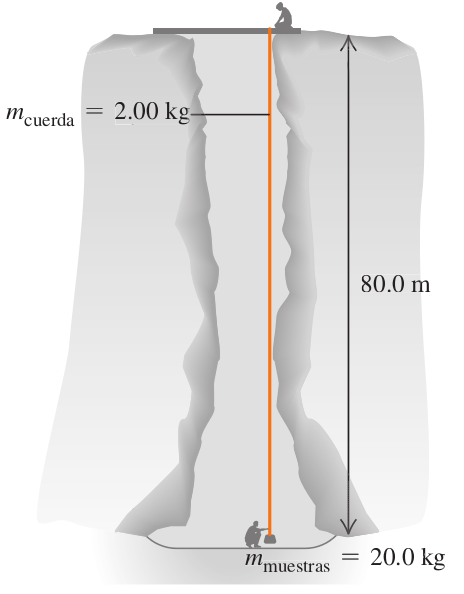
\includegraphics[scale=0.5]{cueva.png}
            \captionof{figure}{ }
            \label{fig:cueva}
        \end{center}
    \end{minipage}

    \pagebreak

    \question Una persona mantiene tenso el extremo de una cuerda de un tendedero y lo mueve hacia arriba y hacia abajo sinusoidalmente, con una frecuencia de 2 Hz y una amplitud de $0.075$ m. La rapidez de onda es $v = 12 \, \frac{\text{m}}{\text{s}}$. En $t = 0$, el extremo en manos de la persona tiene desplazamiento positivo máximo y está en reposo por un instante. Suponga que ninguna onda rebota del extremo lejano. 
    \begin{parts}
        \part Calcule la amplitud de onda $A$, la frecuencia angular $\omega$, el periodo $T$, la longitud de onda $\lambda$ y el número de onda $k$.
        \part Obtenga una función de onda que la describa. 
        \part Escriba las ecuaciones para el desplazamiento, en función del tiempo, del extremo del tendero que la persona sujeta y de un punto a 3 m de ese extremo.
    \end{parts}

    \question Un alambre con masa de 40 g está estirado de modo que sus extremos se encuentran fijos en puntos separados 80 cm. El alambre vibra en su modo fundamental con frecuencia de 60 Hz y amplitud en los antinodos de 0.300 cm. 
    \begin{parts}
        \part Calcule la rapidez de propagación de las ondas transversales en el alambre. 
        \part Calcule la tensión en el alambre. 
        \part Determine la velocidad y aceleración transversales máximas de las partículas del alambre.
    \end{parts}

\end{questions}

\end{document}